\section{KAN}
Kolmogorov-Arnold networks are more expressive than their basic formulation from the Kolmogorov-Arnold representation theorem. 
According to the theorem, the layer requirements are two layers, with a corresponding depth of \(2n+1\) and \(n\). However, in practice, we can design networks with different topologies by adding layers or changing the definition of each layer \cite{KAN}. The key idea is to stack layers from the input to the output.

\subsection{Structure}
With these premises, we can construct various topologies of Kolmogorov-Arnold networks by simply stacking layers and following these rules:
\begin{itemize}
    \item A KAN, as all MPLs, is a directed acyclic graph (DAG). 
    \item Each KAN layer is fully connected to the preceding and succeeding layers apart from the first layer will only have a succeeding layer and the last layer will only have a preceding layer.
    \item Each KAN layer is not connected with other layers
    \item Each KAN layers connection $\textbf{x}_{l+1} = \boldsymbol{\Phi}_L \times \textbf{x}_l$ is defined by $\boldsymbol{\Phi_{L}} \in \Re^{n_{out},n_{in}}$ where $n_{in}$ is the dimension of the $\textbf{x}_l$ layer and $n_{out}$ is the dimension of the $\textbf{x}_l$ layer (Section~\ref{sec:ma}).
    \item Every edge of al layer $\phi_{l,q,p}$ is associated with a one-dimensional activation function. 
\end{itemize}

Let’s say we have a KAN with $L$ layers, where the $l^{th}$ layer has shape $n_{l+1}$, $n_l$ and has formula $\textbf{x}_{l+1} = \boldsymbol{\Phi} \times \textbf{x}_l $. Then the whole network will be represented by:

$$KAN(\textbf{x}) = \boldsymbol{\Phi_{L-1}} \times \dots \times \boldsymbol{\Phi_{1}} \times \boldsymbol{\Phi_{0}} \times \textbf{x}$$

We can also rewrite the above equation as a series of summations, assuming the output dimension $n_L = 1$ and the associated multivariate
continuous function $f$:  $f(x) \equiv KAN(x)$:

$$f(\textbf{x}) = \sum_{i_{L-1}=1}^{n_{L-1}}  \phi_{L-1,i_L,i_{L-1}} (...(\sum_{i_1=1}^{n_{1}}  \phi_{1,i_2,i_{1}}(\sum_{i_0=1}^{n_{0}}  \phi_{0,i_1,i_{0}}(x_{i_0}))...)$$

The network structure will be only a series of matrix-matrix multiplication of $ \boldsymbol{\Phi_{L-1}}, \dots, \boldsymbol{\Phi_{1}},\boldsymbol{\Phi_{0}}$  while a MLPs was a series of linear transformations $W_l$ and non-linear transformations $\sigma$:

$$MLP(\textbf{x}) = \boldsymbol{W_{L-1}} \times \sigma \times \dots \times \boldsymbol{W_{1}} \times \sigma \times\boldsymbol{W_{0}} \times \textbf{x}$$

\begin{figure}[H]
    \centering
    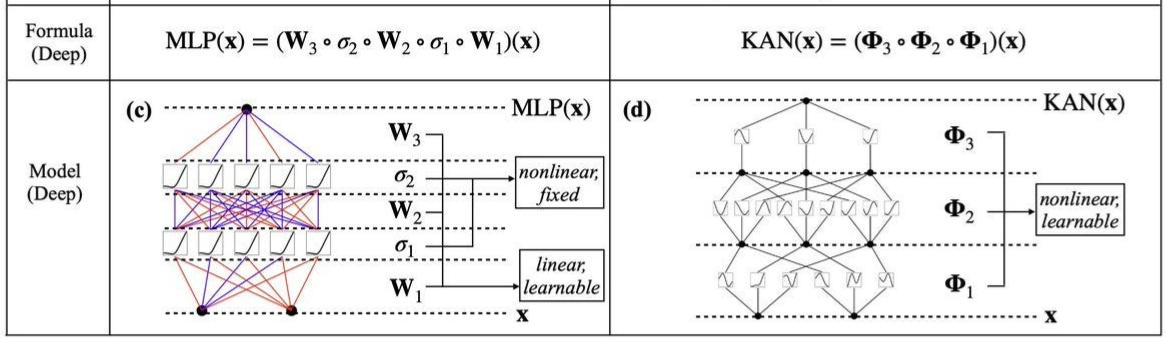
\includegraphics[width=0.8\linewidth]{Images/B.JPG}
    \caption{ MLPs vs KANs: Deep model }
\end{figure}

Finally, a KAN can be conceptualized as a structured stack of KAN layers. Each KAN layer can be represented as a fully connected layer where every edge is associated with a one-dimensional (1D) function. The critical components that need to be defined are the representation and training of these activation functions which are the only learnable part of the function.

\subsection{Activation functions}
While the equation to compute, given an input, the KAN's output appears very simple, ensuring that the activation functions are well-trained is more complex. The most efficient technique involves leveraging spline functions. These functions are particularly effective for approximating the complexity and the non-linearities of the 1D functions associated with the KAN layers. This approach enhances both the flexibility and trainability of the network \cite{KAN}.

Formally speaking, in KANs, every activation function $\phi_{l,q,p}(\cdot)$ is defined as follows:
$$\phi(x) = w_bb(x) + w_sspline(x) $$

where:
\begin{itemize}
    \item $w_b$ and $w_s$ are learnable weights; in principle are redundant since they can be absorbed into $b(x)$ and $spline(x)$, we still include these factors to better control the overall magnitude. In particular, $w_s$ is very useful to scale the spline function.
    \item $b(x)$ is a fixed function called residual connection function defined by the silu function $b(x) = silu(x) = \frac{x}{1+e^{-x}}$. It is the counterpart of biases in MLPs.
    \item $spline(x)$ that is the learnable function where the real power of KANs came from. In most of the cases is parametrized as a linear combination of B-splines functions ($B_i$) and defining $c_i$s the learnable B-splines points and $k$ is the spline order $spline(x)= \sum_i^k c_iB_i(x)$.
\end{itemize}
